\chapter{Ocena użyteczności}

\begin{comment}
OCENA PRZYDATNOSCI UZYTECZNOSCI WALIDACJA
\end{comment}

Coś ogólnie o tym że ważna jest weryfikacja a w systemach webowych ważne jest badanie użyteczności interfejsu no albo to niżej że poddany dwokrotnie to tutaj opisać że nastąpiła taka potrzeba 

\section{Metodyka badań}

System został dwukrotnie poddany weryfikacji środowiskowej. Pierwszy etap badań odbył się po ukończeniu implementacji pierwszego prototypu systemu. Drugi etap odbył się po ukończeniu drugiego prototypu, który poprawiał niedoskonałości odkryte podczas pierwszego badania.

Do weryfikacji wytypowane zostały dwie funkcjonalności istotne dla działania systemu. Pierwszą z nich jest proces, który musi przejść każdy nowy użytkownik systemu, czyli tworzenie profilu zawodnika. Drugą z wybranych funkcjonalności jest dopasowywanie rywali oraz rzucanie im wyzwania. Jest to najważniejsza funkcja systemu zawierająca elementy interfejsu wymagające weryfikacji użyteczności.

Badania odbyły się w formie badań moderowanych[?], czyli z udziałem osoby nadzorującej ich przebieg. Moderatorem w przypadku wszystkich badań był autor tej pracy. Rolą moderatora w przypadku takich badań jest obserwacja akcji podejmowanych przez osobę wykonującą zadania w systemie oraz sporządzanie notatek.

Do badań zostały wybrane osoby potencjalnie zainteresowane tematem, czyli osoby uprawiające sporty zespołowe. W celu zbadania użyteczności systemu dla różnych grup wiekowych zaproszono osoby w przedziale od 15 do 35 lat. Wśród ankietowanych były osoby profesjonalnie zajmujące się systemami webowymi jak również osoby spoza tej branży. Zgodnie z zaleceniami odnalezionymi w literaturze, w każdym z etapów badań wzięło udział pięciu respondentów[?].

Dla uczestników badania została przygotowana ankieta składająca się z trzech części. Pierwsza część była ankietą wstępną uzupełnianą przed badaniami. Zawierała ona krótkie wprowadzenie do systemu oraz pytania<>. Kolejne dwie części zawierały opisy zadań przygotowanych dla użytkowników oraz pytania kontrolne dotyczące intuicyjności poszczególnych procesów. 

Uczestnicy badania zostali poinformowani o tym, że obiektem badania jest interfejs systemu, a nie oni sami. Ze względu na obecność moderatora osoby uczestniczące w badaniu zostały poproszone o głośne myślenie oraz wyrażanie uwag. Moderator podczas badań na bieżąco notował istotne akcje podejmowane przez użytkowników oraz ich uwagi. Po wykonaniu zadań miała miejsce krótka dyskusja na temat napotkanych problemów w obsłudze oraz potencjalnych usprawnień. Na podstawie notatek moderatora zostały sporządzone protokoły (odwołanie do załącznika) oraz wyciągnięte wnioski dotyczące dalszego rozwoju interfejsu.

\section{Przebieg i wyniki badań}

W pierwszej kolejności do systemu zostały wprowadzone przykładowe (zmyślone) dane zawodników, drużyn oraz obiekty sportowe. Umożliwiło to wykonanie testów wymagających interakcji z innymi obiektami w systemie.

W poniższych sekcjach został opisany przebieg oraz wyniki badań poszczególnych funkcjonalności systemu. Szczegółowe wyniki w postaci złożonych ankiet oraz sporządzonych protokołów można znaleźć w załączniku (odniesienie).

\subsection{Tworzenie profilu zawodnika}

W ramach pierwszego zadania ankietowani zostali zalogowani na przygotowane konta użytkowników w systemie, a następnie poproszeni utworzenie profilu zawodnika. Krokami prowadzącymi do wykonania zadania było odnalezienie odpowiedniego formularza a następnie wypełnienie go. 

Poniżej zostaną opisane czynności, na których użyteczność moderator zwracał szczególną uwagę podczas badania.

\subsubsection{Odnalezienie funkcjonalności}

Użytkownicy nie mieli problemów z odnalezieniem kreatora zawodnika. Dwie osoby zasugerowały, że formularz mógłby pokazywać się od razu po pierwszym logowaniu do systemu. Uwaga ta została wzięta pod uwagę podczas implementacji drugiego prototypu.

\begin{figure}[ht]
\centering
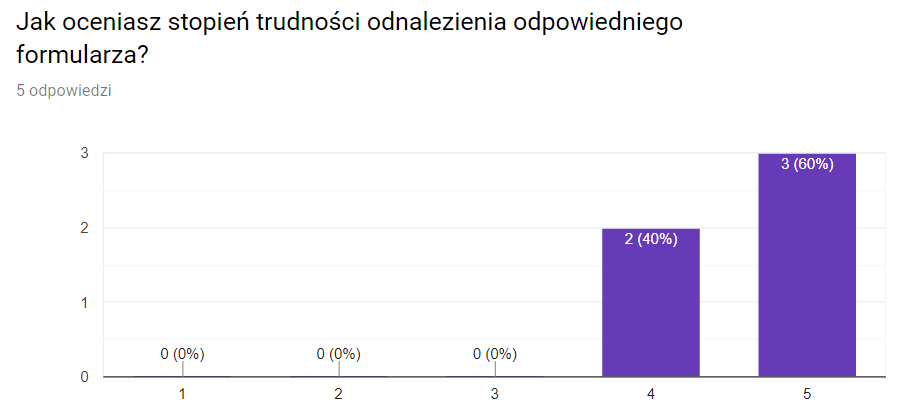
\includegraphics[width=0.95\linewidth]{07-walidacja/rys/profil_trudnosc_odnalezienia.PNG}
\caption{Zestawienie ocen trudności odnalezienia formularza tworzenia zawodnika po pierwszym etapie badań (1 - bardzo trudne, 5 - bardzo łatwe)}
\label{fig:view-player-skill}
\end{figure}


\subsubsection{Nawigacja po formularzu}

Nawigacja po formularzu składającym się z paru kroków nie sprawiła żadnych problemów respondentom.


\begin{figure}[H]
\centering
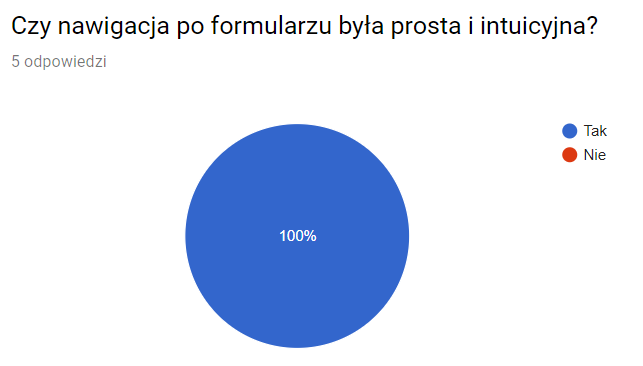
\includegraphics[width=0.7\linewidth]{07-walidacja/rys/p_nawigacja.PNG}
\caption{Aaaaaa}
\label{fig:view-player-skill}
\end{figure}

\subsubsection{Deklaracja poziomu umiejętności}

  Również krok polegający na deklaracji poziomu umiejętności nie stanowił żadnych trudności. Każdy z ankietowanych był w stanie czytając opisy poszczególnych profili umiejętności dopasować się do jednego z nich. Dokonywanie wyborów poprzez przesunięcie suwaków było w pełni intuicyjne.
  
  
\begin{figure}[H]
\centering
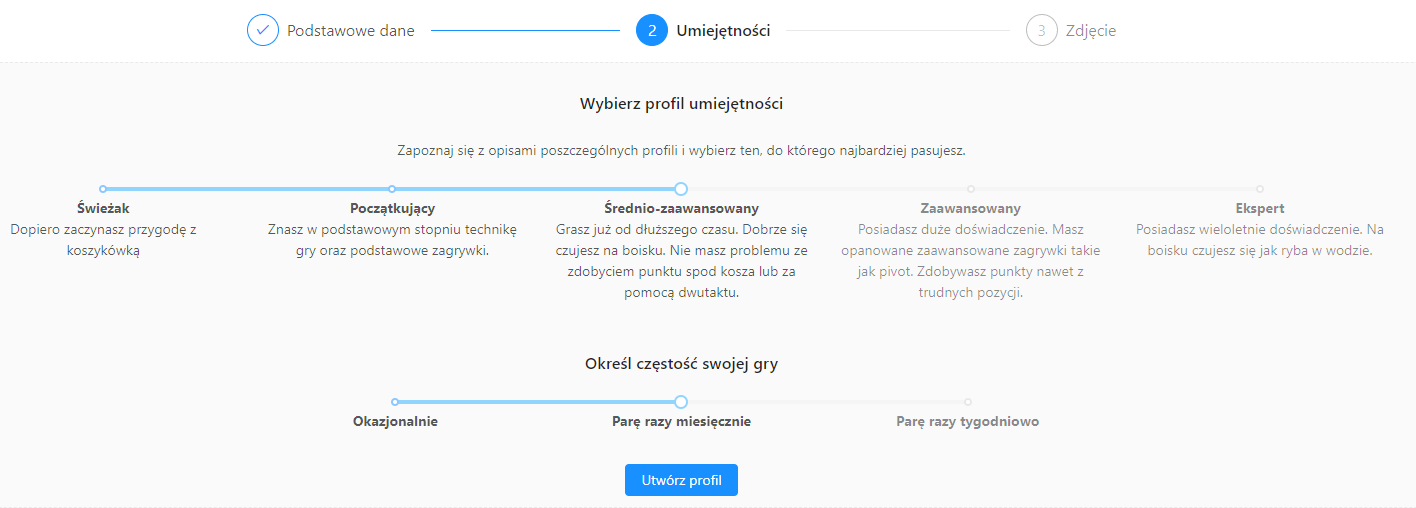
\includegraphics[width=\linewidth]{07-walidacja/rys/p_skill.PNG}
\caption{Aaaaaa}
\label{fig:view-player-skill}
\end{figure}

\subsection{Szukanie przeciwników i rzucanie wyzwania}

Drugie zadanie 

\subsubsection{Odnalezienie funkcjonalności}

O tym ze moglby byc odnosnik na stronie spolecznosci. O tym ze malo kto zwracal uwage na przycisk "Szukaj rywali" ze wzgledu na jego pozycje.

\subsubsection{Deklaracja preferencji wyszukiwania}

O suwaczkach i ich problemach. O tym ze dodatkowe preferencje bez problemu.

\subsubsection{Wyniki wyszukiwania}

O tym ze jest ok ale wiek moglby byc bezwzgledny.

\subsubsection{Oferty terminu oraz miejsca spotkania}


\subsubsection{Nawigacja}


> Co było badane,
> Widoki,
> na co była zwracana uwaga
> wyniki 1 iteracji
> wnioski
> co poprawione
> wyniki 2 iteracji




\begin{comment}
\subsection{Dodatkowe spostrzeżenia}
> Jeśli potrzebne

> Co było badane,
> Widoki,
> na co była zwracana uwaga
> wyniki 1 iteracji
> wnioski
> co poprawione
> wyniki 2 iteracji
\end{comment}